\part{Progettazione di un'interfaccia grafica per la compressione di immagini}

Abbiamo deciso di realizzare il software per la seconda parte del progetto utilizzando il framework Qt\cite{qt}, che permette di progettare interfacce grafiche scrivendo codice in linguaggio C++. Il nostro programma permette, fondamentalmente, di visualizzare, in tempo reale, il risultato di una compressione definiti il livello di taglio dei blocchi e la dimensione di quest'ultimi. Non è presente una funzionalità di salvataggio dell'immagine perché il nostro non è uno standard riconosciuto e sarebbe, per cui, inutilizzabile in altri programmi.
Idealmente, però, basterebbe progettare la struttura del file in modo da contenere le sequenze dei valori non nulli dei blocchi associata ad altre informazioni generali, come la dimensione reale dell'immagine, la grandezza dei blocchi o la soglia di taglio, per poter scrivere un visualizzatore di immagini che sia in grado di effettuare il parsing di quel file ed eseguire la IDCT2.

Il programma fornisce una schermata nella quale è possibile selezionare l'immagine da comprimere e i valori di compressione da applicare, ossia dimensione dei blocchi e la soglia di taglio delle frequenze. Nella parte sinistra della GUI viene mostrata l'immagine originale, mentre in quella di destra la sua versione compressa. In figura \ref{fig:deer} è riportato un esempio sull'immagine \textit{deer}, sulla quale sono stati applicati blocchi di elevate dimensioni (70x70) ed una elevata compressione (circa del 92\%), in questo modo è facilmente osservabile l'effetto della compressione sui blocchi e sull'immagine.

\begin{figure}[h]
	\centering
	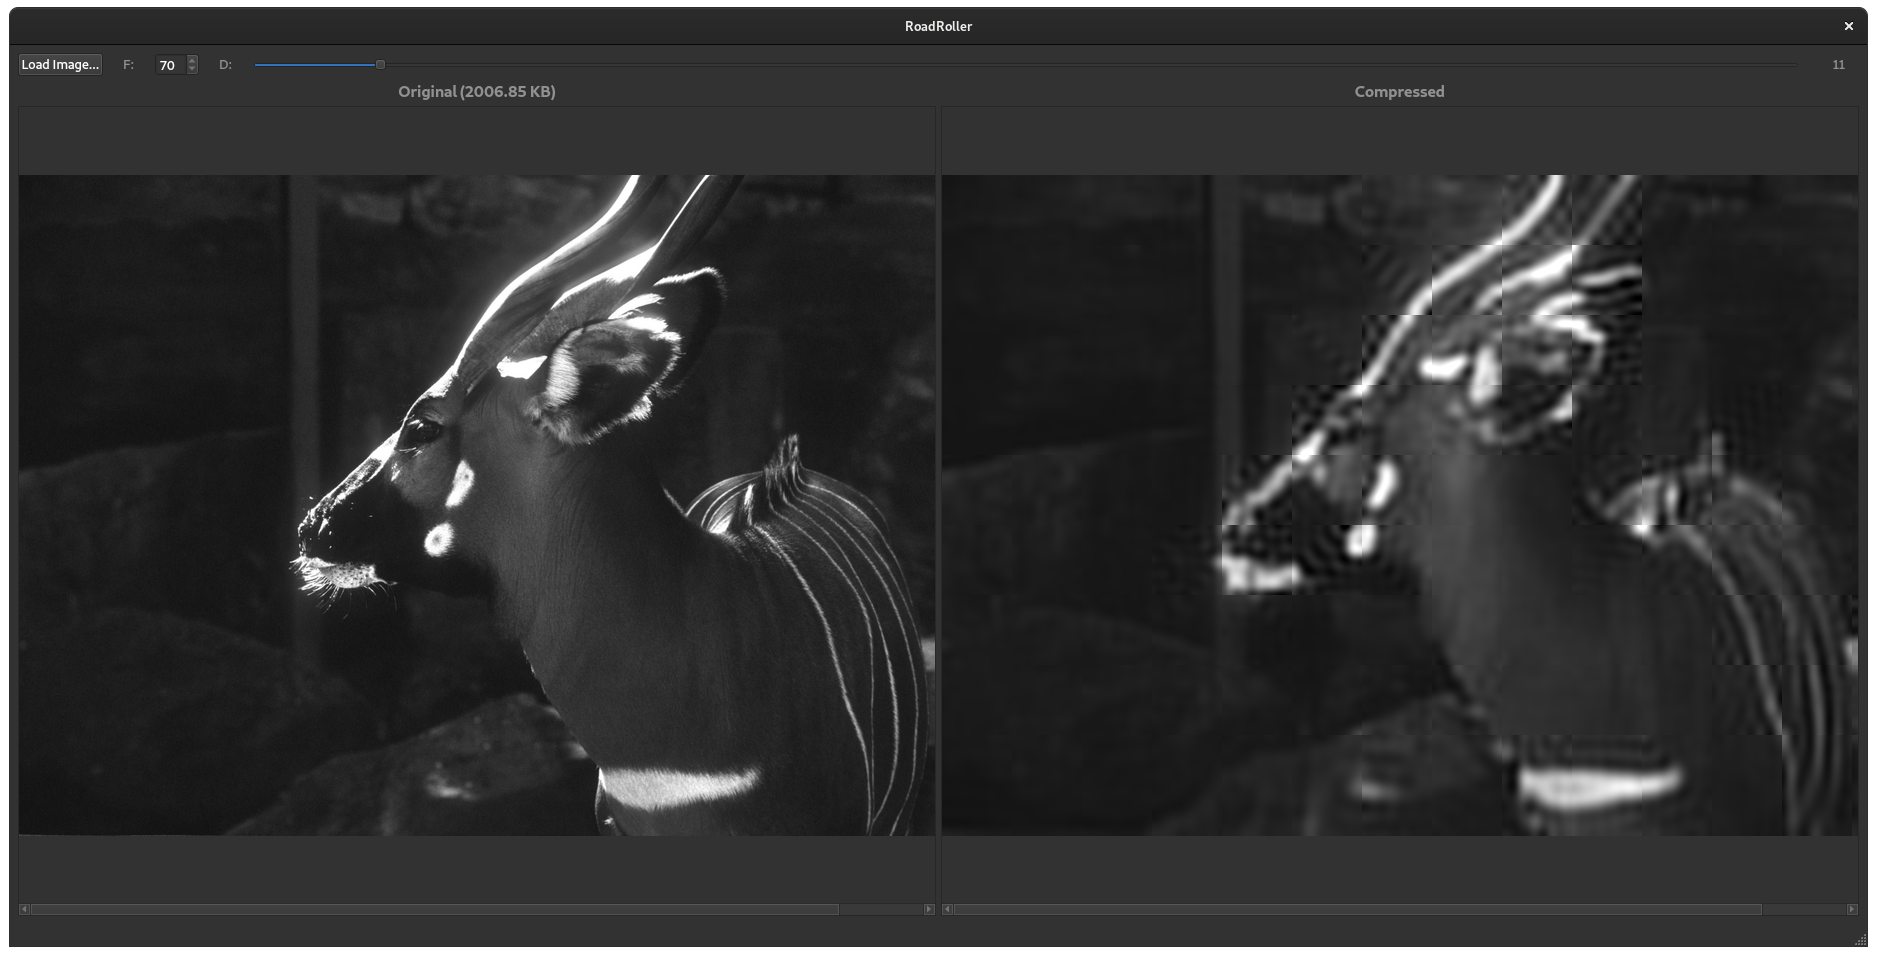
\includegraphics[width=1\linewidth]{figures/qt_deer}
	\caption{Programma di compressione basato su Qt}
	\label{fig:deer}
\end{figure}

Il diagramma delle classi relativo a questo progetto è molto breve, infatti sono state create solamente 2 classi. La prima per gestire l'interfaccia grafica, chiamata \textit{MainWindow}, mentre la seconda, \textit{BlockManager}, si occupa della gestione dei blocchi e la loro relativa compressione. In questo caso, a differenza del primo progetto, vi è meno la necessità di creare  un'architettura con più classi in quanto la funzionalità è unica e precisa. Abbiamo, comunque, fatto in modo che la classe relativa alla finestra GUI sia separata dalla logica di compressione delle immagini al fine di cercare di mantenere una certa \textit{separation of concerns}. Questo diagramma viene mostrato in Figura \ref{fig:class_diagram}.


\begin{figure}[h]
	\centering
	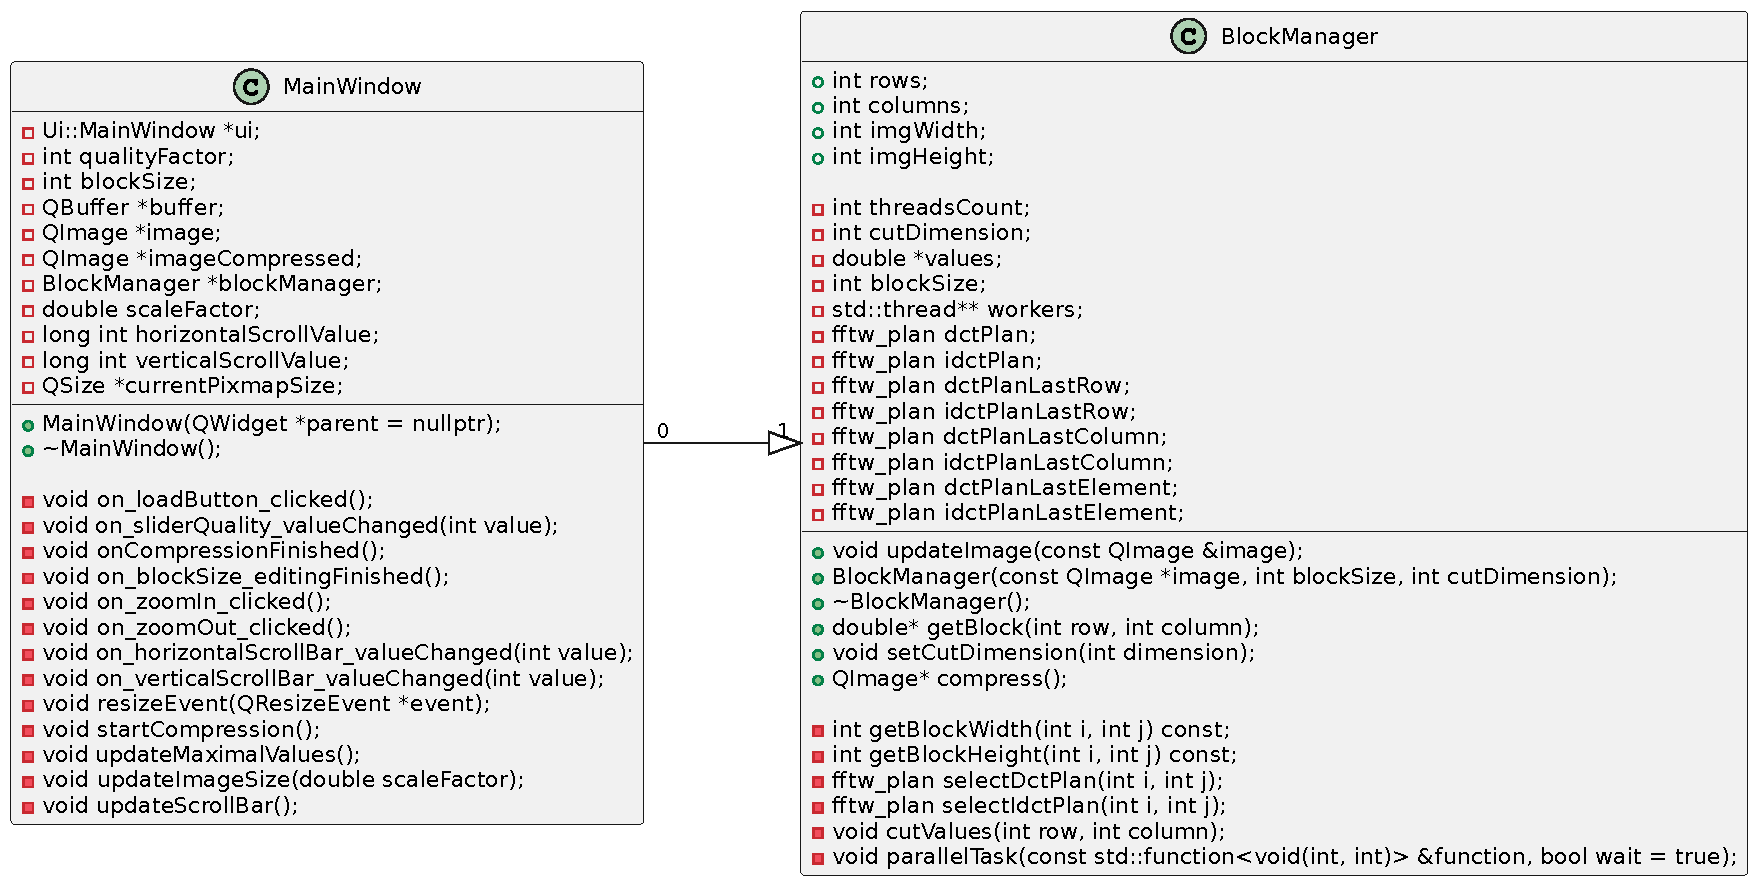
\includegraphics[width=1\linewidth]{figures/class diagram}
	\caption{Diagramma delle classi}
	\label{fig:class_diagram}
\end{figure}

\section{Features}

Alla versione base del progetto, descritto precedentemente, sono state aggiunte un insieme di funzionalità:

\begin{itemize}
	\item \textbf{Multithreading}: L'aggiunta dei thread permette una rapida compressione dell'immagine. Infatti essendo che i blocchi lavorano su aree della figura indipendenti gli uni dagli altri, è possibile eseguire le compressioni in parallelo, così come la scrittura dei pixel nell'oggetto immagine finale.
	
	Abbiamo fatto in modo che l'immagine venisse suddivisa in macroblocchi disgiunti tra loro, ognuno contenente un insieme di blocchi $F \times F$ dell'immagine. La cardinalità di questo insieme di macroblocchi è pari circa al numero di core/thread del processore su cui verrà eseguito il nostro programma di compressione. In questo modo, è possibile bilanciare il livello di parallelismo sulla base delle capacità della macchina di parallelizzare i task.
	
	In particolare, per rendere più trasparente possibile ai thread le nostre funzioni, abbiamo creato un metodo chiamato \path{parallelTask}, che prende in input semplicemente una lambda function che ha come argomenti le coordinate "logiche" del blocco all'interno dell'immagine. Ad esempio, si può eseguire parallelamente una qualasiasi funzione in questo modo:
	\begin{lstlisting}[gobble=1]
	parallelTask([&](int i, int j){
		// Fai qualcosa con il blocco (i, j)
		// mentre gli altri thread lavorano su altri blocchi...
	});
	\end{lstlisting}
	
	
	\item \textbf{Navigazione nell'immagine}: All'interno dell'interfaccia grafica sono presenti degli slider e dei tasti per zoomare nelle immagini. Questi tasti sono sincronizzati in modo tale da poter visionare contemporaneamente le stesse zone delle 2 immagini. In questo modo si possono osservare più comodamente i vari effetti che la compressione comporta sulle immagini.
	\item \textbf{Aggiornamento in tempo reale}: Abbiamo costruito l'interfaccia grafica in modo che l'utente possa regolare e visualizzare in tempo reale la compressione dell'immagine, anche su zone particolari (ad esempio, dopo uno zoom). Grazie al parallelismo, inoltre, siamo riusciti a migliorare la latenza di questa operazione.
	\item  \textbf{Gestione dei bordi}:  A fini sperimentali, abbiamo provato ad implementare il processo di compressione in modo che venisse effettuata la DCT anche su blocchi di dimensioni inferiori, composti dagli scarti derivati dalla suddivisione in blocchi di dimensione $ F \times F$. Ulteriori informazioni su questa prova sono presenti alla Sezione \ref{sec:border}.
	
	\item \textbf{Ottimizzazione delle allocazioni di memoria}:
	FFTw prende in input un puntatore ad un'area di memoria contigua di $N \times M$ elementi ed esegue la DCT organizzando per righe il blocco passato. Se le celle di memoria di un blocco sono, però, contigue, questo non è più vero guardando la disposizione dei pixel del  blocco associato all'interno dell'immagine; questo ci aveva inizialmente portato ad allocare i blocchi singolarmente in una classe dedicata. Tuttavia, una sequenza molto grande di piccole allocazioni risultava particolarmente lenta, specialmente su immagini molto grandi. Il parallelismo, in questo caso, non può aiutare in quanto le allocazioni di memoria richiedono l'acquisizione di un lock da parte dei thread, peggiorando ulteriormente la situazione.
	
	Abbiamo pensato, perciò, di organizzare un mapping che permettesse di capire, a partire da un array di blocchi contigui in memoria, a quale pixel dell'immagine corrisponde un certo blocco e viceversa, richiedendo così una sola allocazione di memoria per l'intera immagine. Con questa soluzione, abbiamo incrementato significativamente la performance in fase di caricamento dell'immagine, poiché invece di tante allocazioni quanti sono i blocchi ne viene richiesta solo una. Il tempo di caricamento dell'immagine \textit{bridge} con $F=2$ è passato, per esempio, da qualche decina di secondi ad un tempo quasi istantaneo.
	\end{itemize}

\section{Gestione dei pixel in eccesso}\label{sec:border}

All'interno di questo progetto, abbiamo deciso in modo "sperimentale" di gestire in maniera leggermente diversa da jpeg i pixel sui margini.

Nello specifico, il nostro programma di compressione considera i pixel in eccesso derivati dalla suddivisione in blocchi e li utilizza per creare dei blocchi più piccoli, al fine di riempire l'intera immagine. Dopo questa operazione, ne esegue la DCT2 allo stesso modo degli altri blocchi. Prima di eseguire il taglio, però, la soglia di azzeramento delle frequenze viene adattata in modo da essere proporzionato alla minore quantità di frequenze e da rendere, quindi, la compressione dell'immagine più uniforme:

\begin{equation}
d' = \begin{cases}
	0 &\text{se $d=0$}\\
	\max \left\{  \ceil*{d  \sqrt{ \frac{W \cdot H}{F^{2}}}}, d - \left(F - \min \left\{W , H \right\}\right)   \right \} &\text{altrimenti}
 \end{cases}
 \label{eq:d}
\end{equation}

dove W e H rappresentano rispettivamente la larghezza e l'altezza del blocco preso in considerazione.
La prima espressione del massimo è utile perché, quando il valore della soglia di taglio è piccola, i blocchi sui bordi  non seguirebbero un andamento iniziale della qualità simile a quello dei blocchi centrali, per via della dimensione ridotta che causa un minor numero di frequenze da analizzare. L'espressione successiva fa in modo che, quando $d$ aumenta, venga fatto combaciare il vertice in basso a destra del blocco piccolo con quello degli altri blocchi.

Abbiamo preso questa decisione perché, a differenza di jpeg, non siamo stati vincolati dalla matrice di quantizzazione e abbiamo potuto, quindi, sperimentare una gestione leggermente diversa del margine dell'immagine.


\begin{figure}
	\begin{minipage}{0.5\textwidth}
		\begin{center}
		
			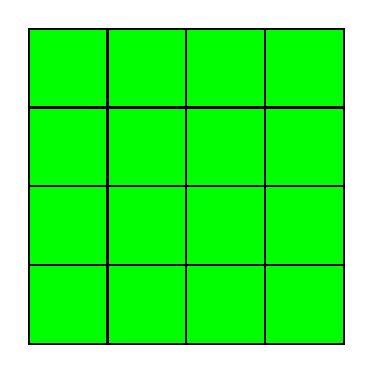
\begin{tikzpicture}
				[%%%%%%%%%%%%%%%%%%%%%%%%%%%%%%
				box/.style={rectangle,draw=black,thick, minimum size=1cm},
				]%%%%%%%%%%%%%%%%%%%%%%%%%%%%%%
				
				\foreach \x in {0,1,...,3}{
					\foreach \y in {0,1,...,3}
					\node[box, fill=red] at (\x,\y){};
				}
			
			
				\foreach \x in {0,...,3}{
					\foreach \y in {0,...,3} {
						\ifnumcomp{\x + (3 - \y)}{<}{5}{
							\node[box, fill=green] at (\x,\y){};
						}{};
					}
				}
				
				
			\end{tikzpicture}
		\end{center}
		\begin{center}
			(a)
		\end{center}
	\end{minipage}\hfill
	\begin{minipage}{0.5\textwidth}
		\begin{center}
			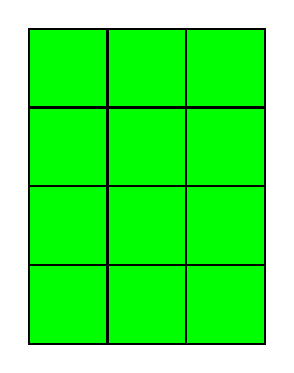
\begin{tikzpicture}
				[%%%%%%%%%%%%%%%%%%%%%%%%%%%%%%
				box/.style={rectangle,draw=black,thick, minimum size=1cm},
				]%%%%%%%%%%%%%%%%%%%%%%%%%%%%%%
				
				\foreach \x in {0,1,...,2}{
					\foreach \y in {0,1,...,3}
					\node[box, fill=red] at (\x,\y){};
				}
				
				
				\foreach \x in {0,...,2}{
					\foreach \y in {0,...,3} {
						\ifnumcomp{\x + (3 - \y)}{<}{4}{
							\node[box, fill=green] at (\x,\y){};
						}{};
					}
				}
				
				
			\end{tikzpicture}
		\end{center}
	\begin{center}
		(b)
	\end{center}
\end{minipage}
\caption{Taglio delle frequenze sulle diverse dimensioni dei blocchi per valori di $F=4$ e $d=5$ In questo specifico esempio, la trasformazione della soglia porterebbe $d$ a decrementare di 1.}\label{fig:taglio}
\end{figure}

\section{Esperimenti sulle immagini}
Questa Sezione contiene alcuni degli esperimenti, che riteniamo più interessanti, effettuati utilizzando il nostro software.

\subsection{Visualizzazione dei tagli}
Per fini dimostrativi, abbiamo provato a visualizzare l'output subito dopo il taglio dei blocchi sui quali è stata effettuata una DCT2. In Figura \ref{fig:compression_values} è mostrato il risultato ottenuto. È importante notare che, essendo una DCT, i toni di grigio dei pixel non dicono molto rispetto alla composizione delle frequenze; si possono notare, tuttavia come, effettivamente, siano presenti dei triangoli pieni di valori nulli, ed è proprio qui il vantaggio di comprimere un'immagine in questo modo. In base alla soglia di taglio scelta, il numero di pixel che si potrebbero scrivere su un file per poter visualizzare l'immagine compressa possono arrivare ad un livello significativamente più basso di quello necessario per rappresentare l'immagine non compressa, portando, quindi, ad un decremento significativo della dimensione del file in cui si potrebbe memorizzare un formato simile a questo.

\begin{figure}%
	\centering
	\subfloat[][Immagine originale]{{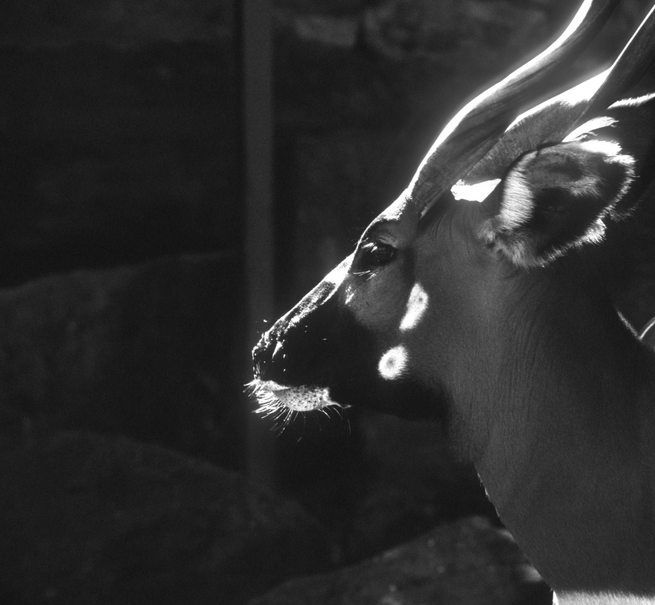
\includegraphics[width=0.49\textwidth]{figures/deer_dct_full.png} }}%
	\subfloat[][Tagli della DCT basati sul valore di $d$]{{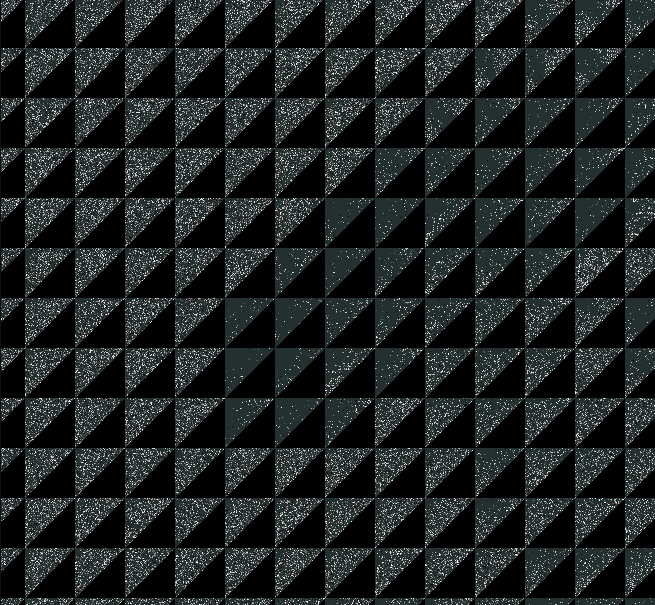
\includegraphics[width=0.49\textwidth]{figures/deer_dct.png} }}%
	\caption{Compressione dell'immagine \textit{deer} per $F=50$ e $d=50$. Si notino i triangoli neri che completano ognuno dei blocchi mostrati.}%
	\label{fig:compression_values}
\end{figure}


\subsection{Fenomeno di Gibbs}

Scegliendo un'elevata dimensione dei blocchi si rende particolarmente visibile il fenomeno di Gibbs, mostrato in Figura \ref{fig:gibbs}. La sua presenza tende ad essere più fastidiosa con blocchi grandi perché è più probabile che, all'aumentare di $F$, aumenta lo spazio all'interno del quale le basse frequenze cercano di compensare la carenza di quelle alte per rappresentare i cambiamenti repentini del tono di grigio presenti nel blocco stesso.

Nelle Figure \ref{fig:dct_values_on_gibbs} e \ref{fig:last_dct_values_gibbs} sono rappresentati rispettivamente l'intero istogramma del blocco mostrato in Figura \ref{fig:gibbs} e un suo zoom sulle ultime $50 \times 50$ frequenze. Nonostante la presenza di basse frequenze sia decisamente maggiore di quella delle alte frequenze, sono proprio quest'ultime che sono in grado di rappresentare al meglio i dettagli e, quindi, anche il bordo superiore della testa del cervo. Al momento del taglio, con un valore di $d$ basso, queste spariscono del tutto e non è, quindi, più possibile mostrare il cambiamento netto dell'immagine originale.

In contrasto, la Figura \ref{fig:gibbs_small} mostra come, la dimensione contenuta dei blocchi (in questo caso, $8 \times 8$), sia sufficiente al fine di limitare il fenomeno a piccolissime aree dell'immagine, rendendolo quasi impercettibile.

\begin{figure}%
	\centering
	\subfloat[][Immagine originale]{{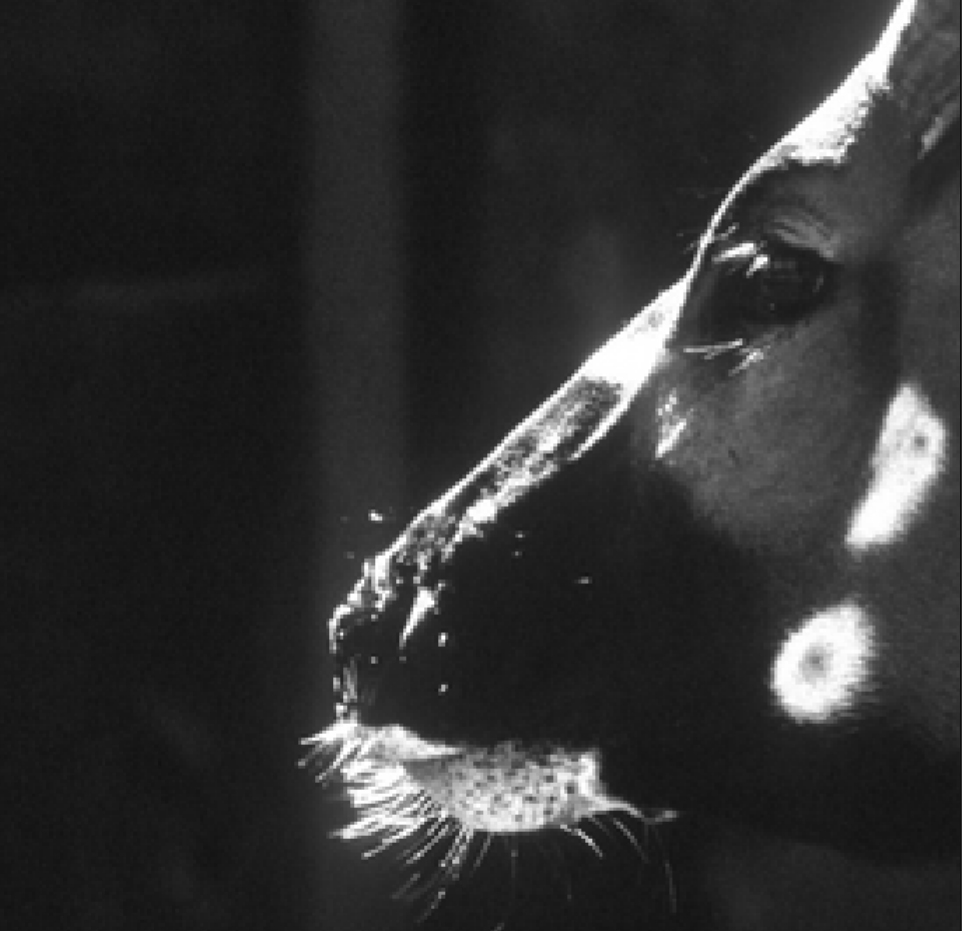
\includegraphics[width=0.49\textwidth]{figures/deer_gibbs_full.png} }}%
	\subfloat[][Immagine compressa]{{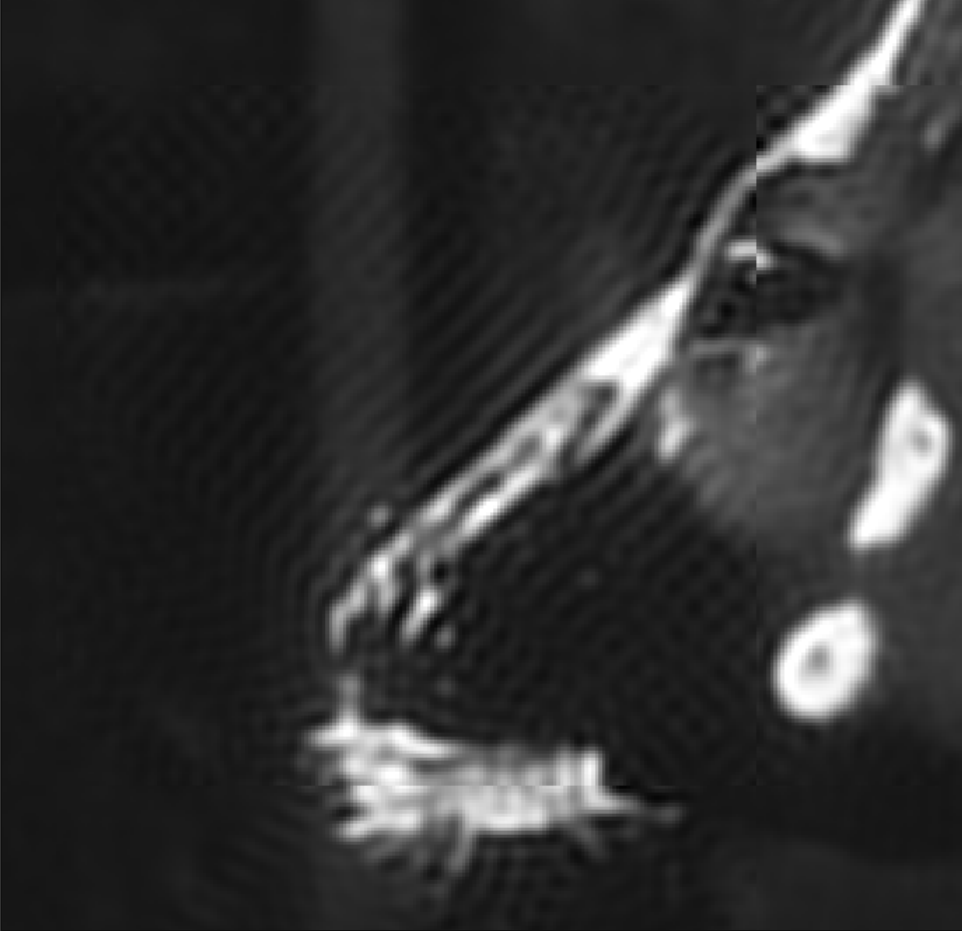
\includegraphics[width=0.49\textwidth]{figures/deer_gibbs_comp.png} }}%
	\caption{Compressione dell'immagine \textit{deer} con $F=200$ e $d=70$. Si può distinguere chiaramento il limite del blocco centrale, che delimita il fenomeno di Gibbs.}%
	\label{fig:gibbs}
\end{figure}

\begin{figure}%
	\centering
	\subfloat[][Immagine originale]{{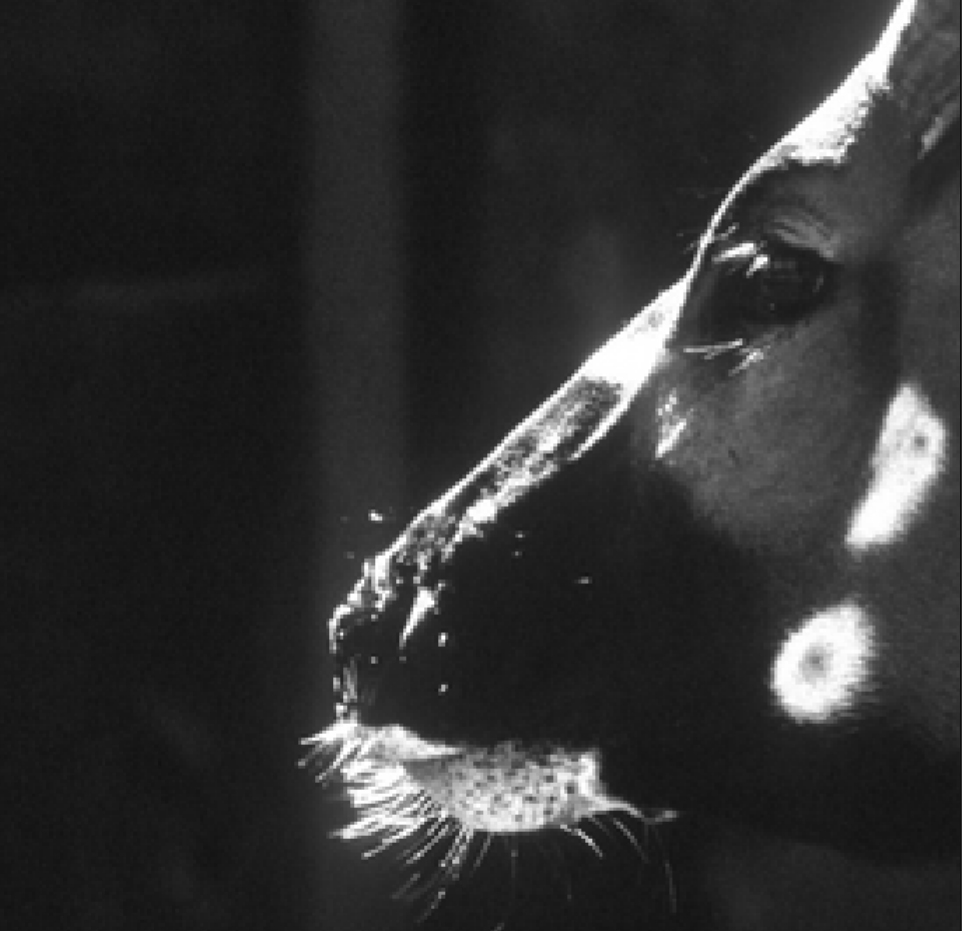
\includegraphics[width=0.49\textwidth]{figures/deer_gibbs_full.png} }}%
	\subfloat[][Immagine compressa]{{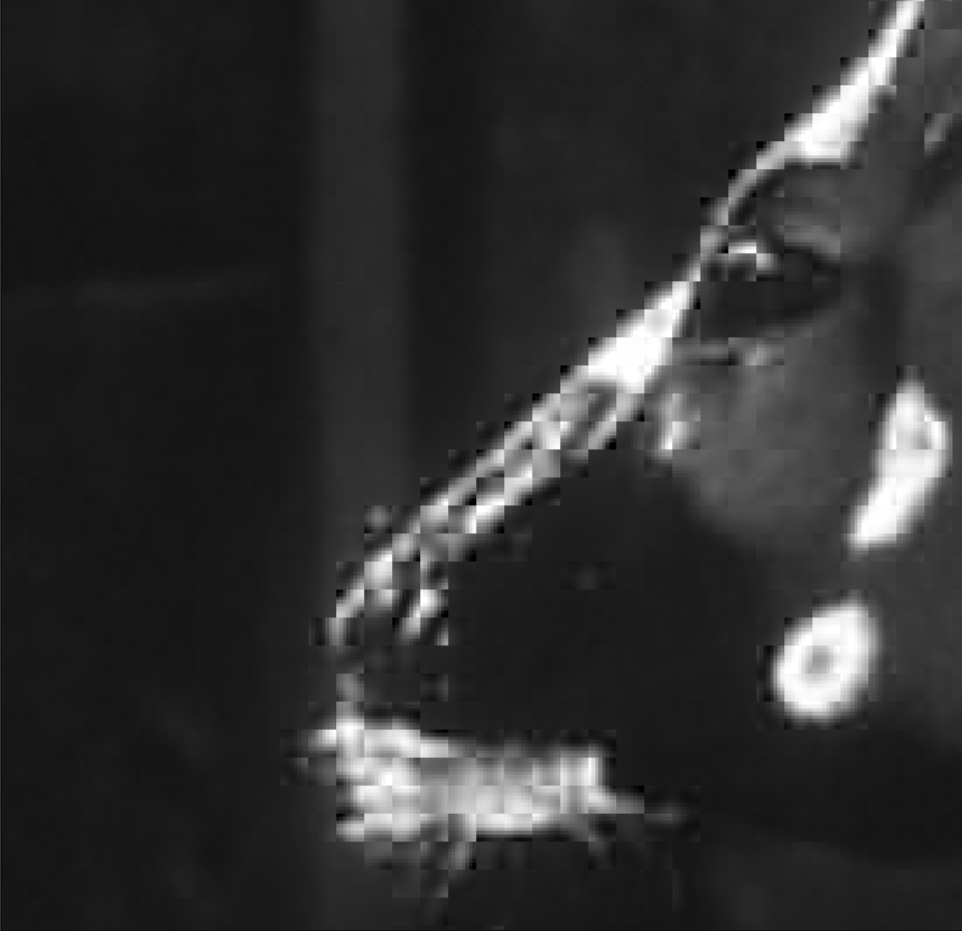
\includegraphics[width=0.49\textwidth]{figures/deer_notgibbs_comp.png} }}%
	\caption{Compressione dell'immagine \textit{deer} con $F=8$ e $d=3$. Il risultato di questa compressione evidenzia come, con blocchi piccoli, sia possibile limitare il fenomeno di Gibbs ad aree molto piccole.}%
	\label{fig:gibbs_small}
\end{figure}

\begin{figure}
	\centering
	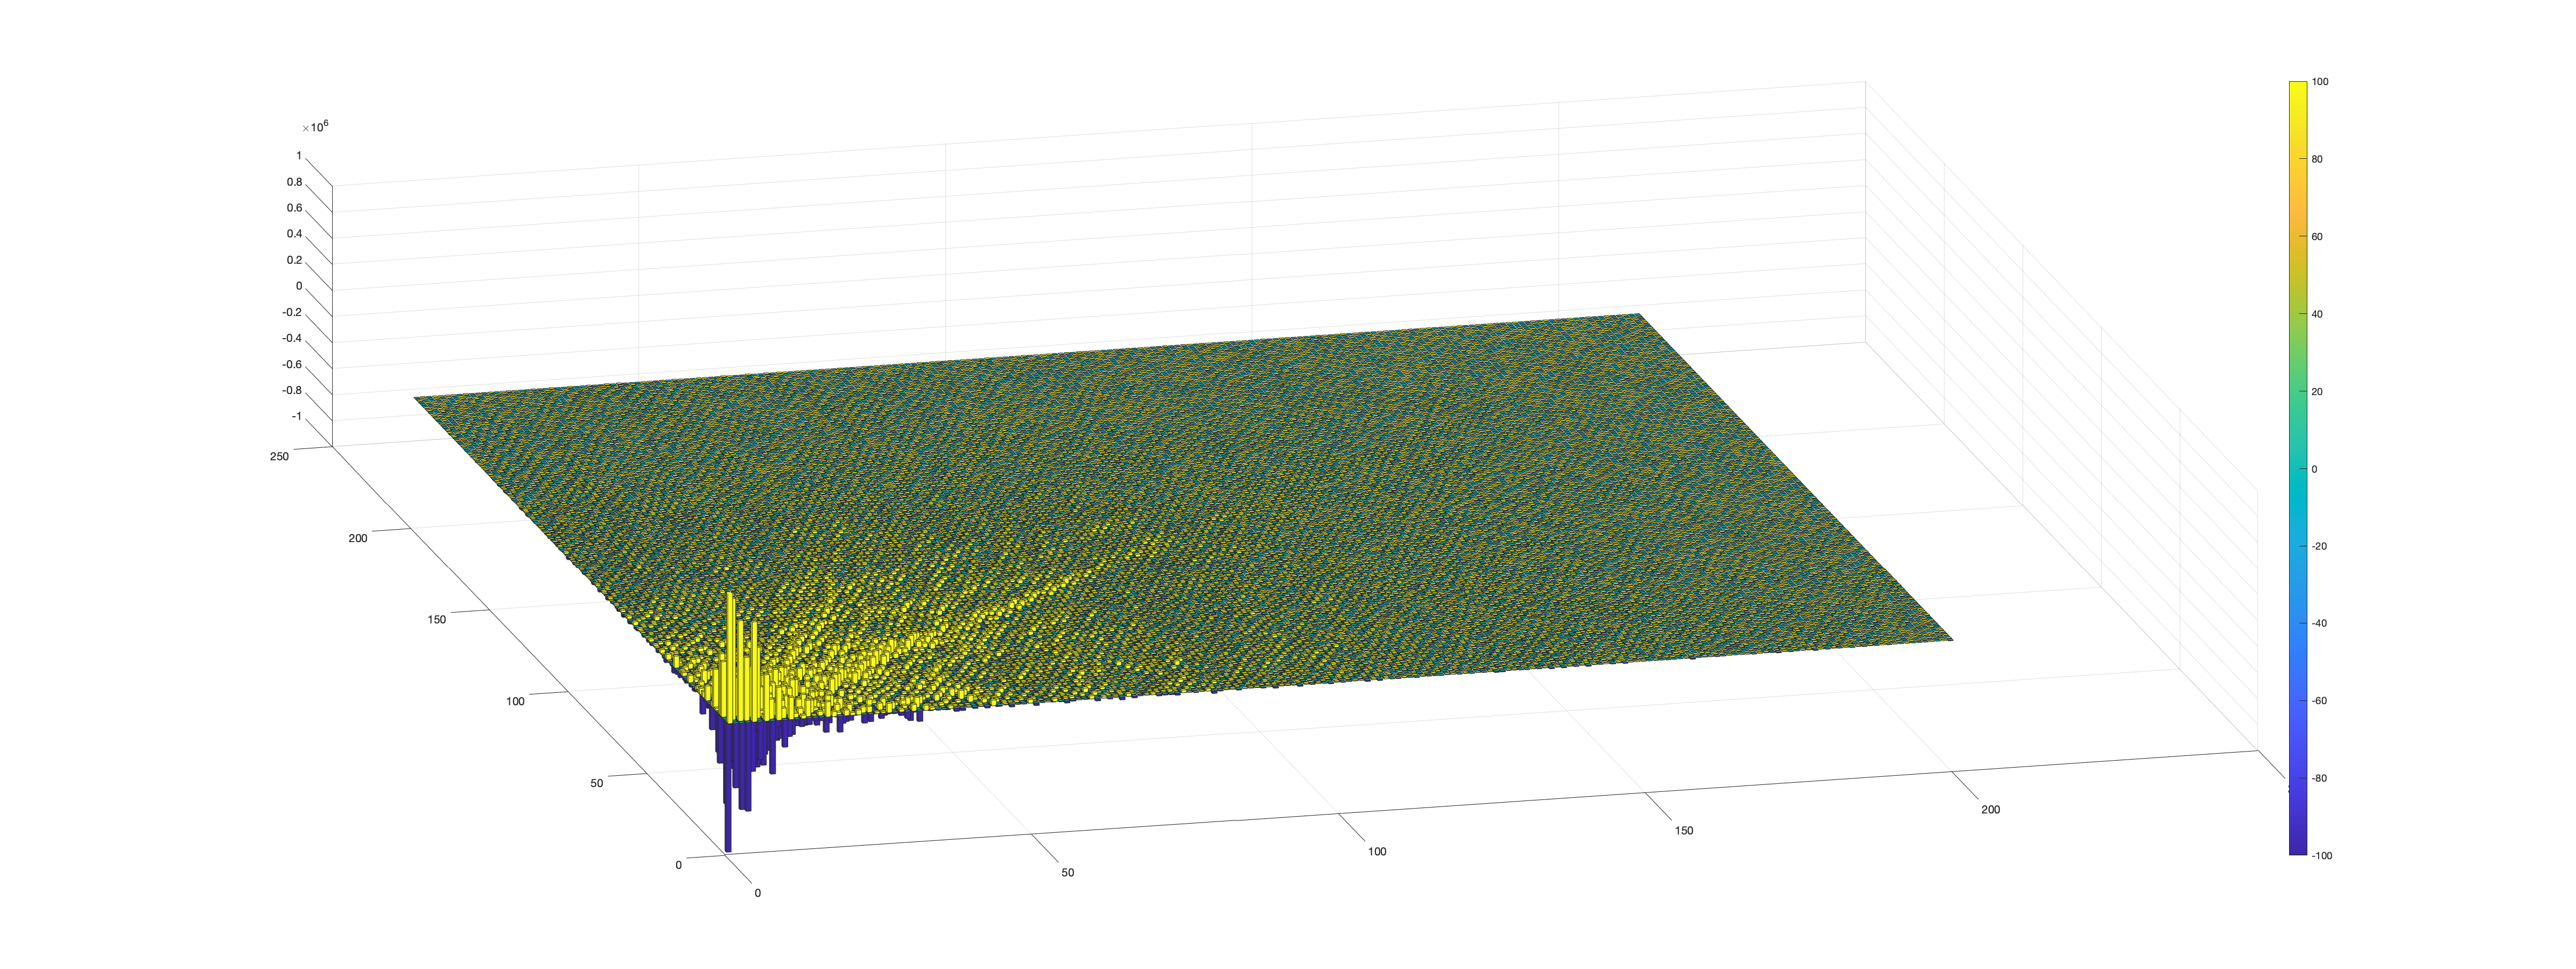
\includegraphics[width=1\linewidth]{figures/dct_values_3d.eps}
	\caption{Coefficienti DCT nel blocco mostrato in Figura \ref{fig:gibbs}}
	\label{fig:dct_values_on_gibbs}
\end{figure}

\begin{figure}
	\centering
	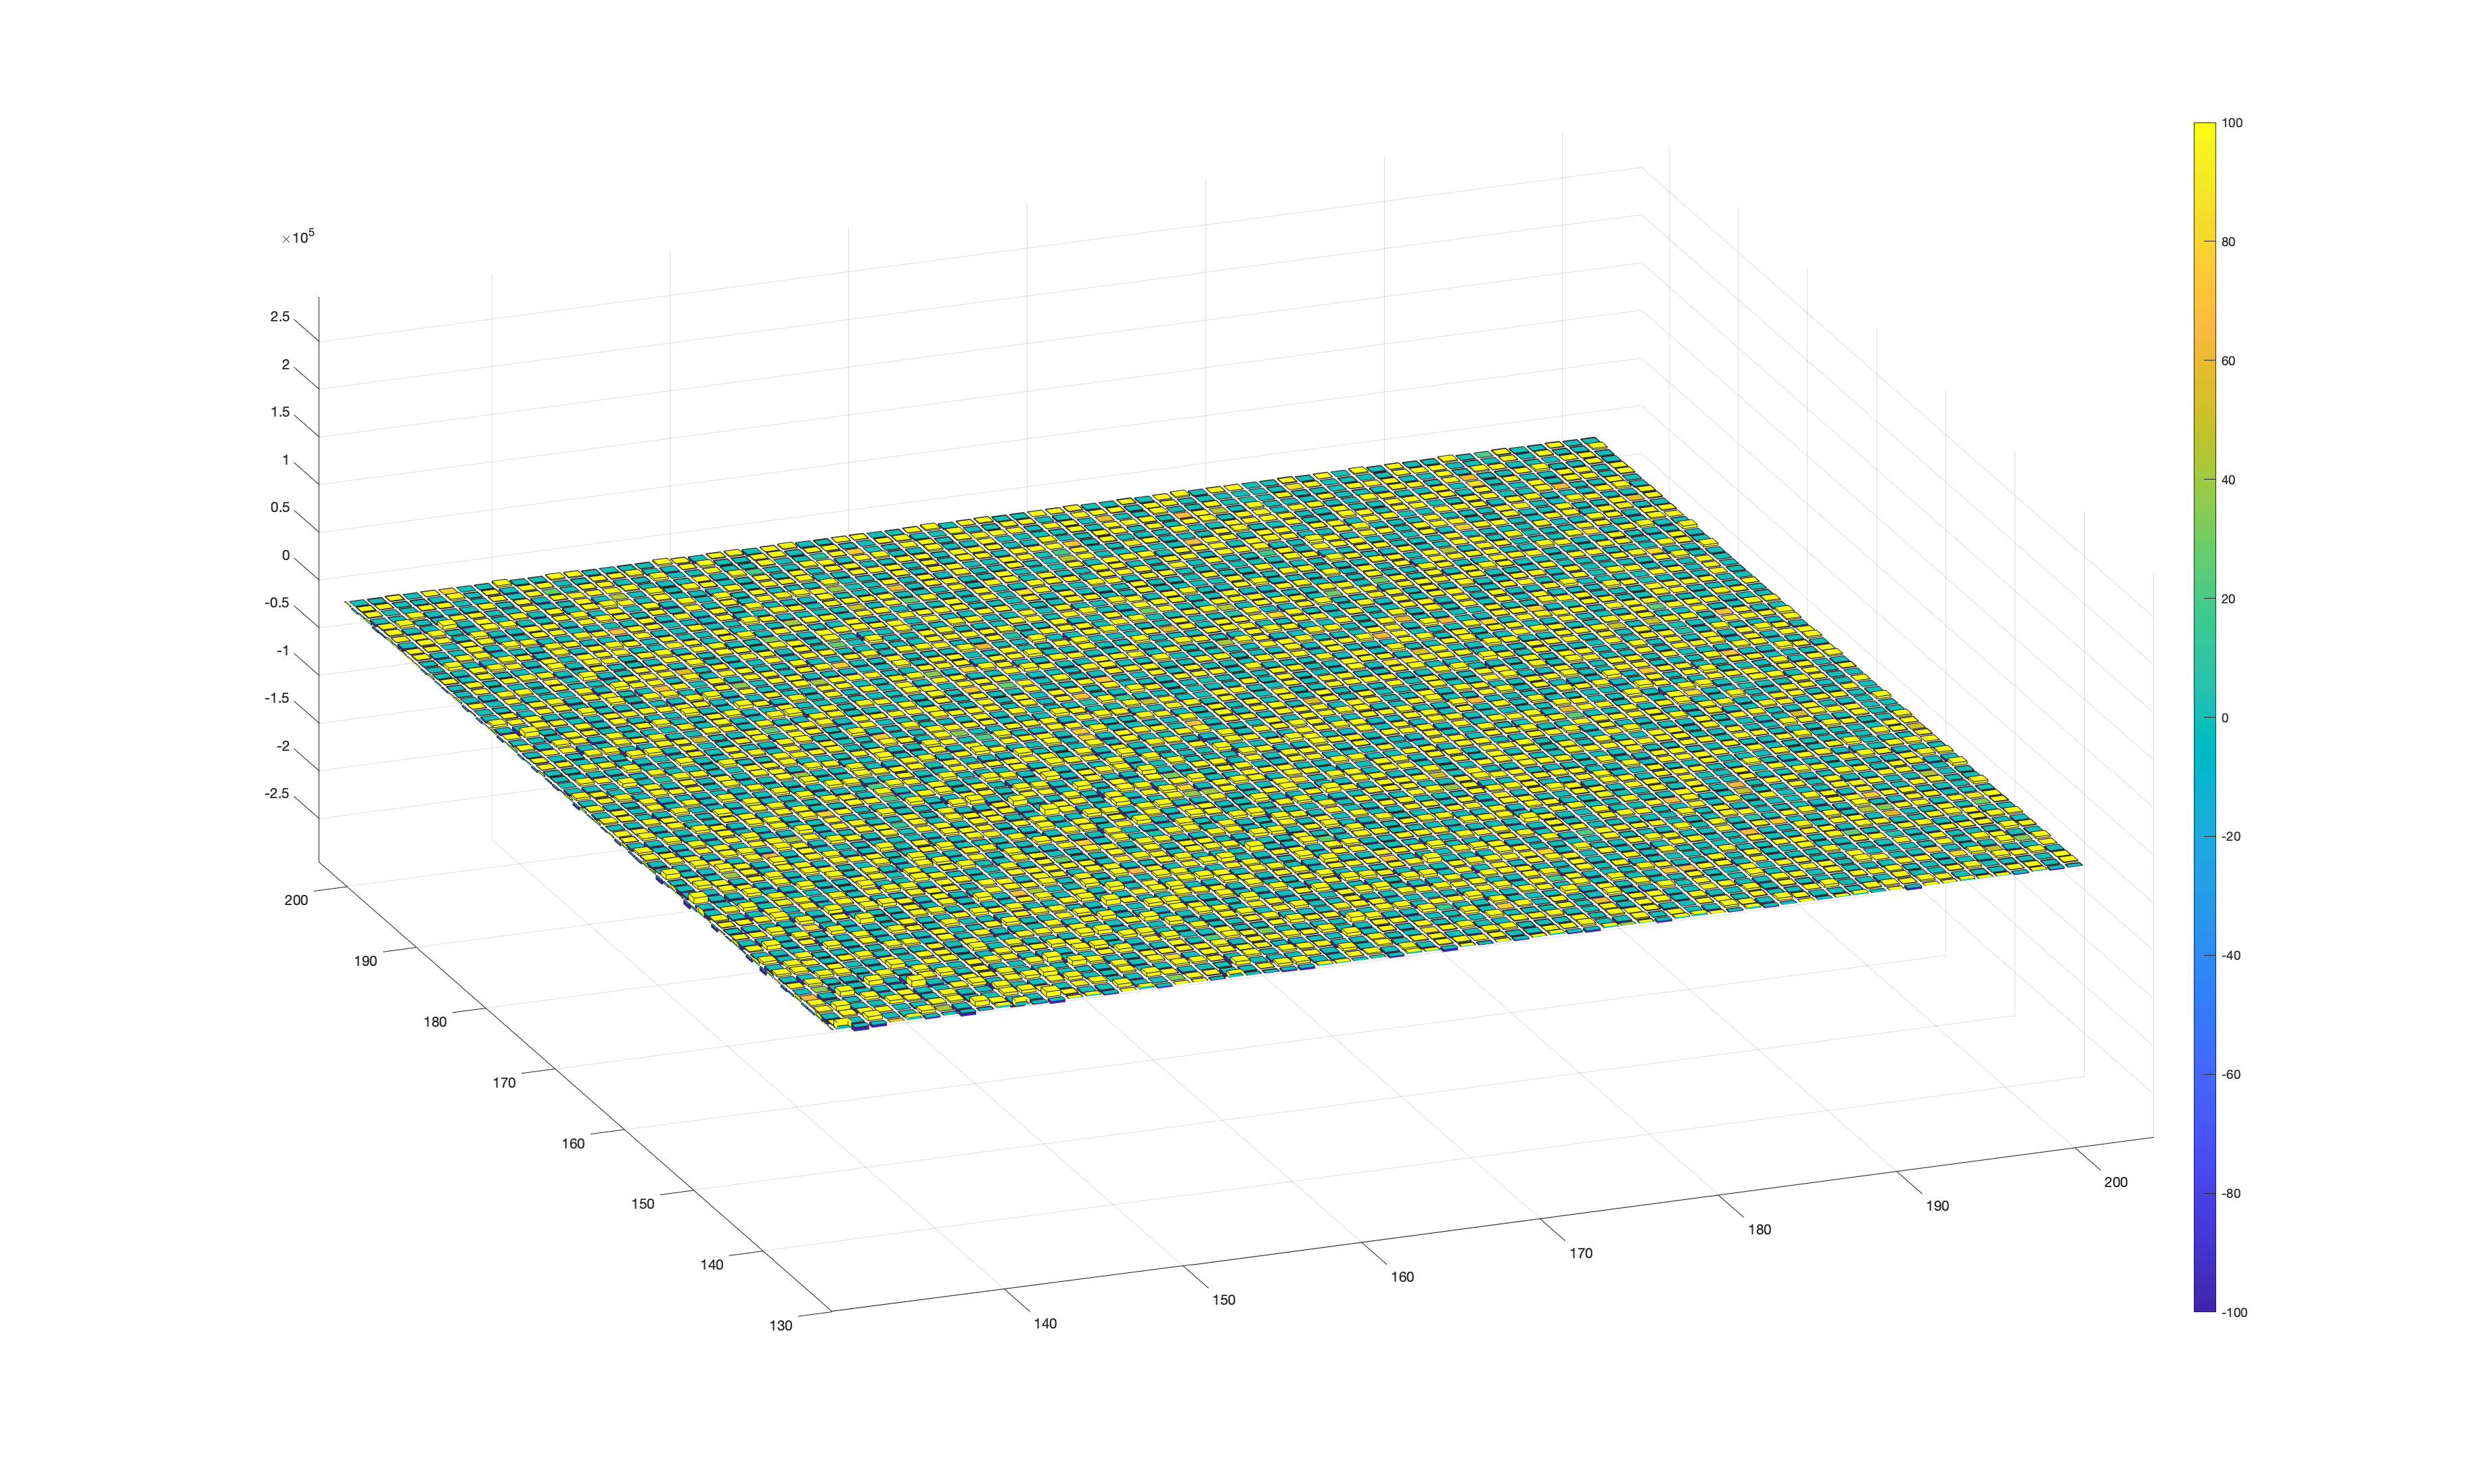
\includegraphics[width=1\linewidth]{figures/last_dct_values.eps}

	\caption{Ultimi 50 x 50 coefficienti della DCT relativi alla Figura \ref{fig:dct_values_on_gibbs}}
	\label{fig:last_dct_values_gibbs}
\end{figure}
\FloatBarrier

\subsection{Caso del gradiente}
\begin{figure}%
	\centering
	\subfloat[][Immagine originale]{{
\includegraphics[width=0.49\textwidth]{figures/gradient_full.png} }}%
	\subfloat[][Immagine compressa]{{
\includegraphics[width=0.49\textwidth]{figures/gradient_comp.png} }}%
	\caption{Compressione dell'immagine \textit{gradient} con $F=100$ e $d=1$}%
	\label{fig:gradient}
\end{figure}

In Figura \ref{fig:gradient} è mostrato l'output della compressione dell'immagine \textit{gradient}. Questo risultato è particolare rispetto agli altri, poiché non si distinguono i blocchi ma si possono vedere distintamente le colonne della DCT. Osservando la costruzione dell'immagine di input, abbiamo un'idea del motivo per cui si è manifestato questo fenomeno: per ogni colonna di pixel, il tono di grigio è costante. Questo vuol dire che, in realtà, la DCT in quella direzione e non ha bisogno di frequenze diverse dalla prima per rappresentare i vettori colonna in modo accurato.

Non presentando transizioni brusche di colori, inoltre, il fenomeno di Gibbs risulta essere molto limitato rispetto a immagini come, per esempio, \textit{deer}.



\subsection{DCT sui blocchi a margine}
Abbiamo anche testato il comportamento dell'algoritmo di aggiustamento di $d$ all'Equzione \ref{eq:d} in una situazione "normale" e in un caso estemo
Facendo qualche esperimento sulle immagini, specialmente quelle a quadrati bianchi e neri, abbiamo notato fondamentalmente due cose:
\begin{enumerate}
	\item Quando la dimensione dei blocchi è relativamente contenuta, la compressione risulta uniforme anche se i blocchi non sono della stessa dimensione di quelli interni;
	\item Nel momento in cui la compressione ha una soglia di taglio bassa e la dimensione del blocco diventa immensa (ad esempio, quasi tutta l'immagine) il risultato della compressione è molto diverso tra la parte interna dell'immagine e quella sui margini. Tuttavia, queesta differenza sparisce nel momento in cui si alza leggermente la soglia di taglio dei valori.
\end{enumerate}
Le due osservazioni sono evidenziate dalle Figure \ref{fig:border_small} e \ref{fig:border_big}. Riteniamo che questo metodo di gestione dei margini funzioni meglio quando i rapporti tra la larghezza e l'altezza di una singolo blocco non sono esageratamente alti,  mentre, nel caso in cui questi lo siano, è necessario un valore di $d$ più alto per arginare il problema. 

Inoltre, osservando l'ultimo blocco in basso a destra, nella Figura \ref{fig:border_big}, si può notare che questo è risultato molto più definito degli altri due. Questo è dovuto alla differenza molto ampia di frequenza da riempire tra questi, rendendo più facile una rappresentazione fedele di esso.


\begin{figure}%
	\centering
	\subfloat[][Immagine originale]{{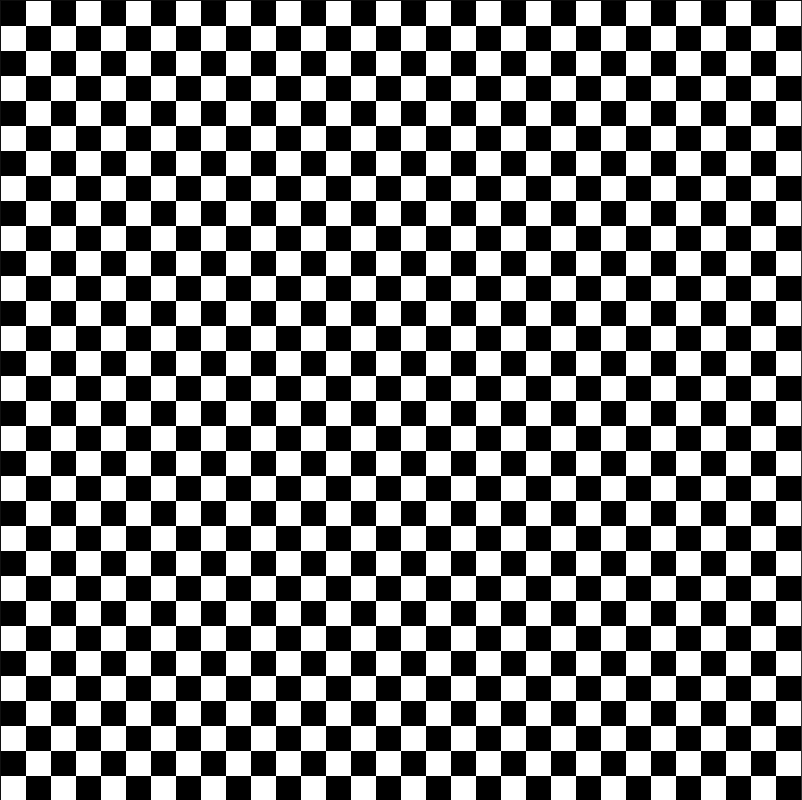
\includegraphics[width=0.49\textwidth]{figures/320.png} }}%
	\subfloat[][Immagine compressa]{{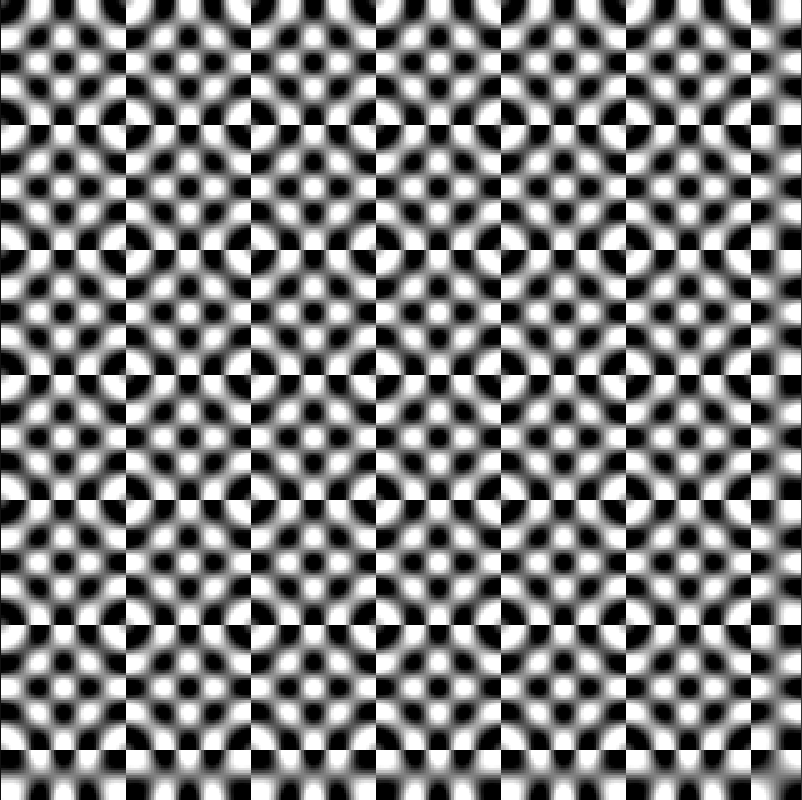
\includegraphics[width=0.49\textwidth]{figures/320_small.png} }}%
	\caption{Compressione dell'immagine $\mathit{320 \times 320}$ con $F=25$ e $d=6$}%
	\label{fig:border_small}
\end{figure}

\begin{figure}%
	\centering
\subfloat[][Immagine originale]{{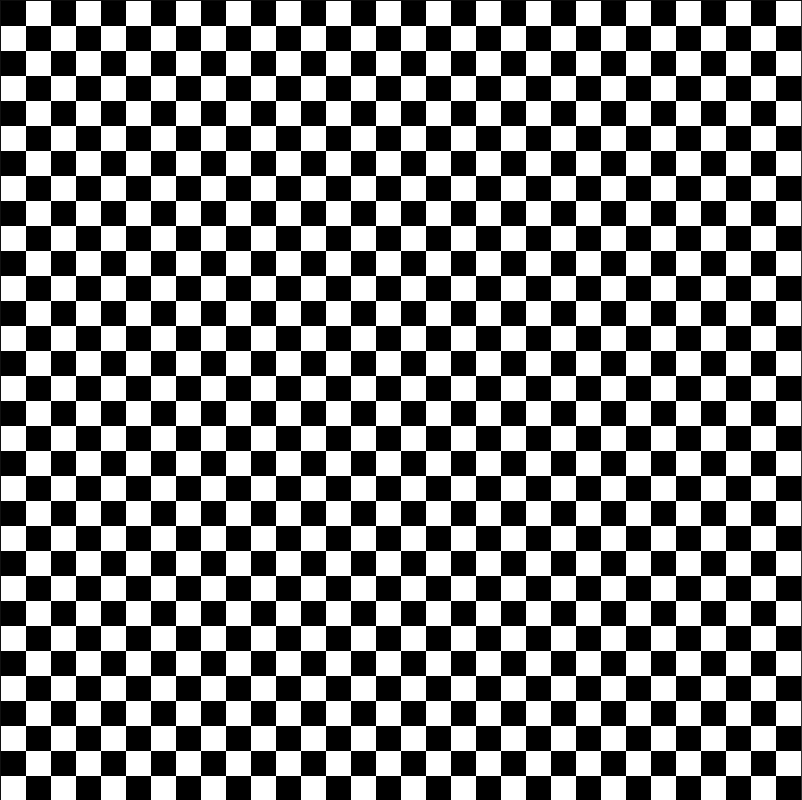
\includegraphics[width=0.49\textwidth]{figures/320.png} }}%
\subfloat[][Immagine compressa]{{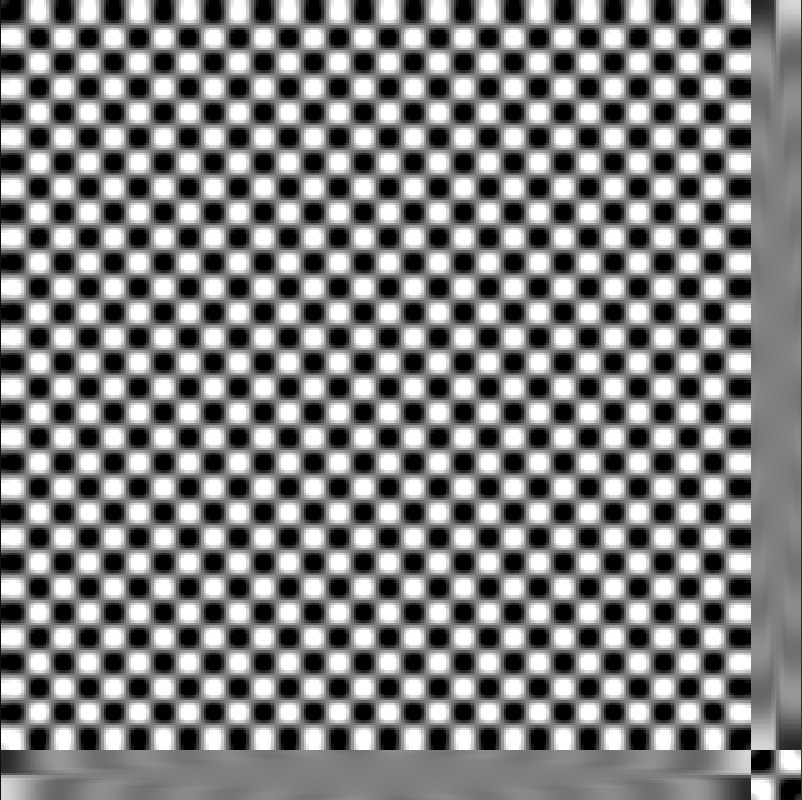
\includegraphics[width=0.49\textwidth]{figures/320_large.png} }}%
	\caption{Compressione dell'immagine $\mathit{320 \times 320}$ con $F=300$ e $d=80$.}%
	\label{fig:border_big}
\end{figure}
